\documentclass[11pt]{article}
\usepackage[margin=24mm]{geometry}
\usepackage{amsmath,amssymb}
\usepackage{tikz}
\usetikzlibrary{arrows.meta}
\begin{document}
\begin{center}
{\Huge A little space to think.}\\[8pt]
{\large Notes on a particle in a potential well}\\[4pt]
\textit{A browser-compiled LaTeX example}
\end{center}
\section{From a sketch to an equation}
Keep the source readable. Your agent can help with the mathematics; the document remains an ordinary \LaTeX{} file.
For a particle of mass $m$, the time-independent Schr\"odinger equation is
\begin{equation}
-\frac{\hbar^2}{2m}\frac{d^2\psi}{dx^2}+V(x)\psi(x)=E\psi(x).
\end{equation}
\begin{center}
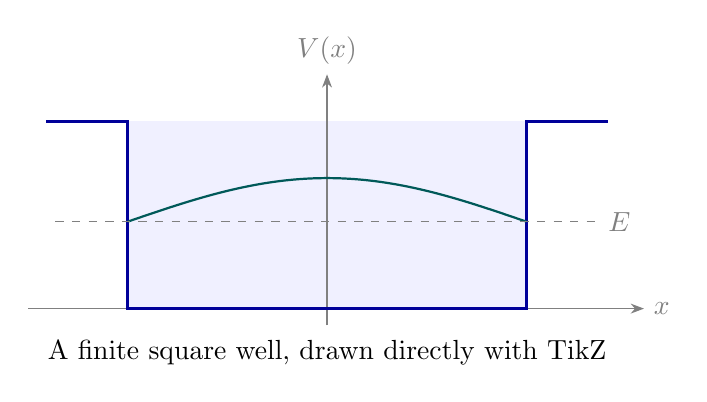
\begin{tikzpicture}[x=1.15cm,y=0.85cm,>=Stealth]
\fill[blue!6] (-2.2,0) rectangle (2.2,2.8);
\draw[->,gray] (-3.3,0)--(3.5,0) node[right] {$x$};
\draw[->,gray] (0,-.25)--(0,3.5) node[above] {$V(x)$};
\draw[very thick,blue!60!black] (-3.1,2.8)--(-2.2,2.8)--(-2.2,0)--(2.2,0)--(2.2,2.8)--(3.1,2.8);
\draw[thick,teal!70!black,domain=-2.2:2.2,samples=80] plot (\x,{1.3+0.65*cos(\x*180/4.4)});
\draw[dashed,gray] (-3,1.3)--(3,1.3) node[right] {$E$};
\node at (0,-.65) {A finite square well, drawn directly with TikZ};
\end{tikzpicture}
\end{center}
\section{A useful approximation}
In a classically forbidden region, a semiclassical estimate gives
\[
T\sim\exp\!\left[-2\int_a^b\frac{\sqrt{2m\,[V(x)-E]}}{\hbar}\,dx\right].
\]
\textbf{Try it:} change the title or the colour of the potential, then compile again.
\paragraph{A note on evidence.} This is synthetic demonstration material. Passage attribution and human review will be added as a separate layer; compilation alone does not establish scientific correctness.
\end{document}
